%!TEX root = ../main.tex

\chapter {Evaluation}
\label {cha:evaluation}
This chapter contains interesting IEC functions and procedures, either found in production code of an industrial partner, collected and translated from literature or were constructed to demonstrate how the implementation works and behaves.
% Each example provides the code, the control flow graph, a description, execution time, number of instruction blocks needed to conclude the result and, most importantly, the reported violations.
Each example provides a description, the code, control flow graph and a visualized directed graph, which visualizes how the implementation executes the analysis. Each example will also be analyzed by the existing tools mentioned in Chapter \ref{cha:state of the art}. In the last Section \ref{sec:overview of results} runtime can be compared with each example.

\section{Infeasible Code Example}
% Beschreibung
The example in Listing \ref{code:basic example 1} and its CFG in Figure \ref{fig:basic example 1 cfg} was found in production code and motivation for this thesis. It does not contain any loops or procedure calls (with the exception of \emph{RESET\_ALARM}, which may be ignored). Two variables of type integer, \emph{m\_operationHour} and \emph{s\_operationHour}, are checked for inequality in lines 1 and 15. The second check in line 15 cannot be reached, since it was already checked before and the function returned. Since neither \emph{m\_operationHour} nor \emph{s\_operationHour} change their value, the second condition will never evaluate too true, resulting in unreachable code in line 16. This assignment will never be executed. 
% Problem
In line 11 an instance of unnecessary code can be observed, because \emph{s\_operationHour} must be equal to \emph{m\_operationHour}, which is 0 in this case. Removing the assignment in line 11 would therefore reduce the number of statements, while it has no effect on the result.

% Ausführung

Figure \ref{fig:basic example 1} illustrates the analysis process. This code is encapsulated in a function and both of the relevant variables do not have a concrete value assigned (it could be any integer), and therefore no state is known at the beginning. The first condition may be true or false and is therefore reachable, which is why both situations have to be considered creating, two branches modeling both possibilities. Following the \emph{then} branch from basic block 1 to basic block 2, the assignment in line 2 equals both variables. Since \emph{s\_operationHour} can still contain any value, the condition in line 3 may still evaluate to either true or false. Whatever the result of this condition is, the function returns afterwards.

Coming back to the first condition in line 1 and following the else branch, both variables must have the same value. The condition in line 9 may evaluate to true or false. If it is true, both variables must be 0 making the statement in line 11 obsolete. When the condition in line 9 is false, the accumulated state from former instructions results in the constraints that both variables must have the same value, which must not be 0. Therefore the condition in line 15 will always result in false and therefore basic block 11 cannot be reached. 

% State of the Art
As described in earlier in Figure \ref{code:Java sonarqube duplicate conditions} the static code analysis tool Sonarqube \cite{sonarqube} does find this instance of infeasible code and reports it as such. As shown in Figure \ref{code:Java intelij duplicate conditions}, IntelliJ \cite{IntelliJIDEACapable} declares this condition as a duplicate condition. But other instances of infeasible conditions may not be found. 

% Relevanz


% 581ms
% 17 Blöcke analysiert
% Violation für block 11

\begin{program}[h!]
	\begin{GenericCode}
IF s_operationHour <> m_operationHour THEN
	m_operationHour := s_operationHour;
	IF s_operationHour = 0 THEN
		RESET_ALARM(Name := er_service, SubID1 := m_iNumber);
	END_IF;
	RETURN;
END_IF;
// s_operationHour must be equal to m_operationHour
IF s_operationHour = 0 THEN
	// unnecessary - already zero
	m_operationHour := 0;
	RESET_ALARM(Name := er_service, SubID1 := m_iNumber);
ELSE
	// unreachable
	IF s_operationHour <> m_operationHour THEN
		s_operationHour := m_operationHour;
	END_IF;
END_IF;
	\end{GenericCode}
	\caption{The example contains one instance of unreachable code in line 16, since the condition always evaluates to false. This is due to the fact that this condition was already checked in line 1, returned in line 6, and since then none of the variables changed their values.}
	\label{code:basic example 1}
\end{program}

\begin{figure}[h!]
	\centering
	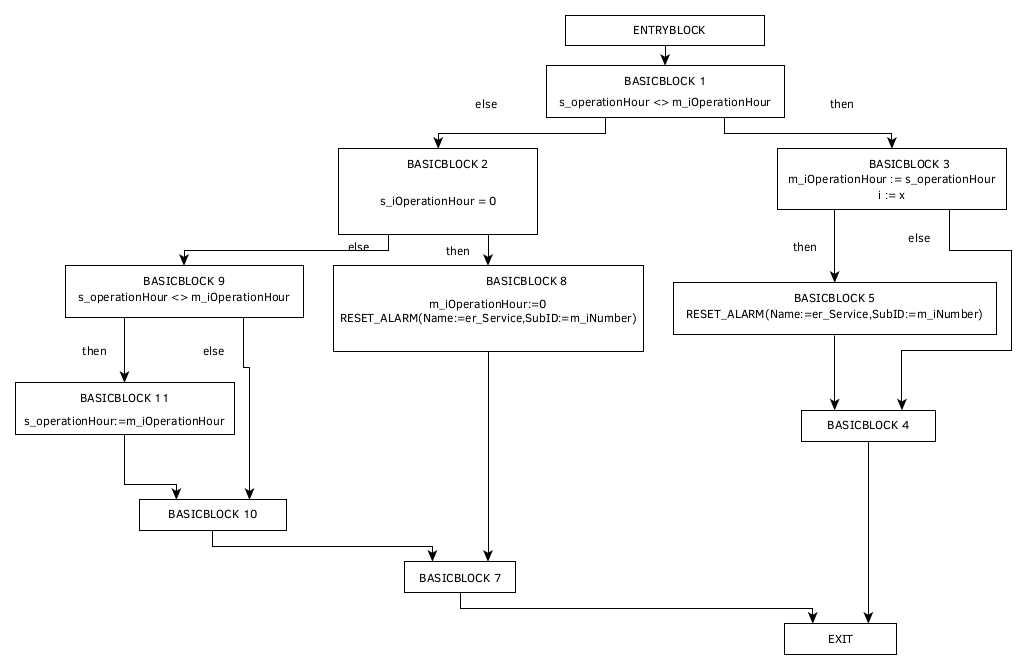
\includegraphics[width=0.9\textwidth]{minimal-example-cfg}
	\caption{Transformed IEC-code into the CFG of Listing \ref{code:basic example 1}. Since all arrows point forward, no loop is present.}
	\label{fig:basic example 1 cfg}
\end{figure}

\begin{figure}[h!]
	\centering
	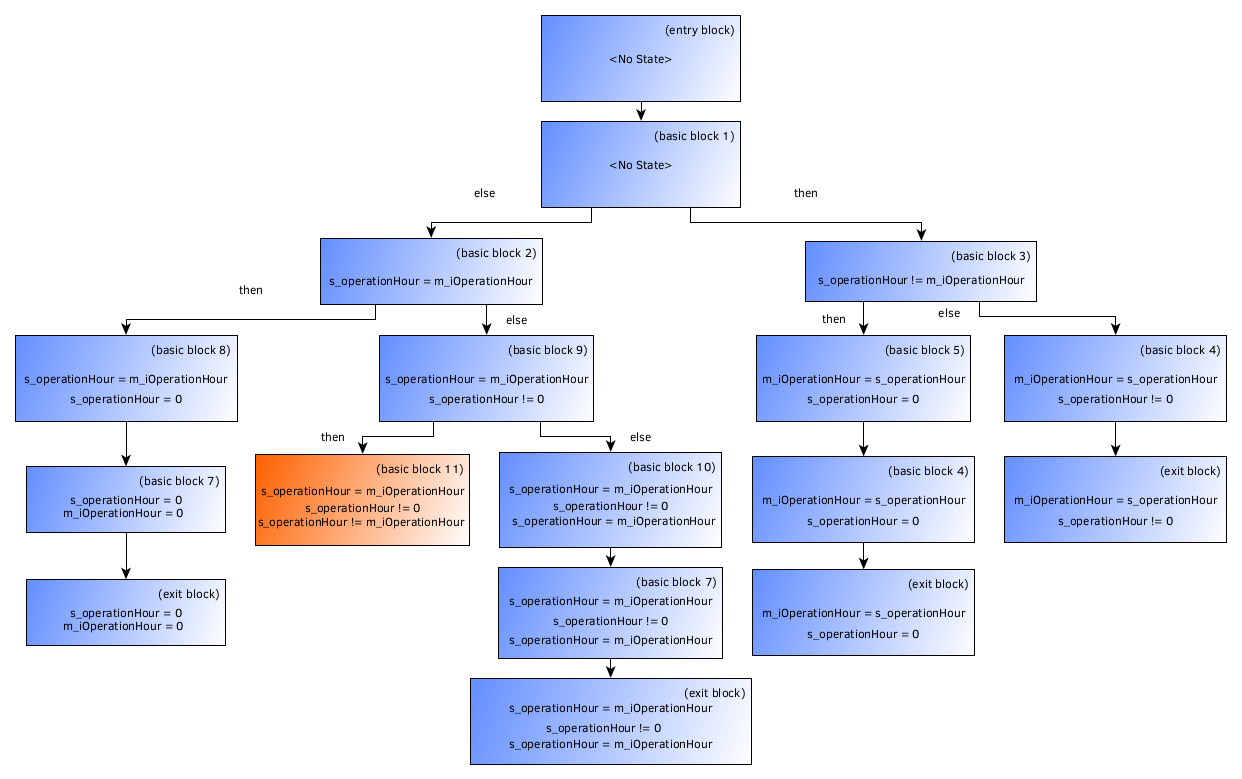
\includegraphics[width=1\textwidth]{minimal-example}
	\caption{Analysis of example shown in Figure \ref{fig:basic example 1 cfg}. As described in Listing \ref{code:basic example 1}, the condition in line 15 always evaluates to false, resulting in unreachable code in line 16, more specifically basic block 11 in Figure \ref{fig:basic example 1 cfg}. }
	\label{fig:basic example 1}
\end{figure}

\section{Loops}
\label{sec:loops}
The examples, seen in Listing \ref{code:loop example 1} and Listing \ref{code:loop example 2}, were created to show the implementation handles simple loops. Both examples do not differ much. The only difference is that the example in Figure \ref{fig:loop example 1 cfg} declares the variable \emph{x} as a local variable, whereas the example in Figure \ref{fig:loop example 2 cfg} declares this variable as input. 
In the first example, the loop will be executed four times and every loop iteration increases the value of variable \emph{i}. Therefore \emph{i} holds the value 5 and the condition in line 8 will always evaluate to false and resulting in unreachable code in line 9 (basic block 6). This can also be observed in Figure \ref{fig:loop example 1}.


The second example will lead to a different result, demonstrated in Figure \ref{fig:loop example 2}, since the value of variable \emph{x} may be of any number. Therefore the number of iterations would also be nondeterministic, as shown in Figure \ref{fig:loop example 1} . But, as described in Section \ref{sub:early stopping}, this analysis will stop, because every statement is reachable, since the value of \emph{x} could be three and therefore \emph{i} evaluates to three. 


The tools covered in Chapter \ref{cha:state of the art} do not find this instance of unreachable code in the first example. Maybe Joogie, described in Section \ref{sec:sca paper} is  able to find it. This is due to the fact that the mentioned tools evaluate loops only once.

\begin{program}[h!]
		\begin{GenericCode}
i := 1;
x := 5;
		
WHILE i < x DO
	i := i + 1;
END_WHILE;
		
IF i = 3 THEN
	x := 4;
END_IF;	\end{GenericCode}
\centering
\caption{A simple loop that increments a number. Since \emph{i} is dependent on the iterations, which are limited by and will be equal to \emph{x}, in this case 5, the condition in line 8 will never evaluate true.}
\label{code:loop example 1}
\end{program}

\begin{figure}[h!]
	\centering
	% 61ms
	% 20
	% Violation für block 6
	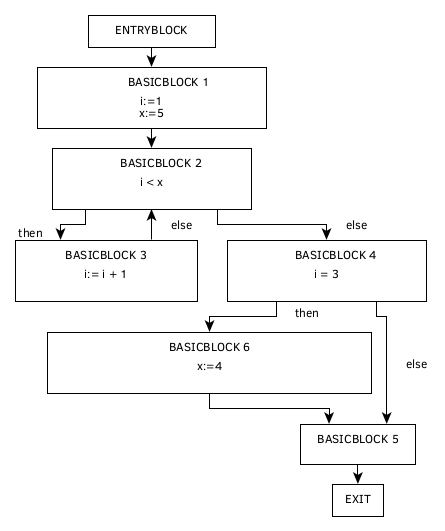
\includegraphics[width=0.6\textwidth]{basic-while-cfg}
	\caption{Transformed IEC-code into the CFG of Listing \ref{code:loop example 1}. As long as x is not equal to 3, the basic block 6 is unreachable. The loop can be observed between the basic blocks 2 and 3.}
	\label{fig:loop example 1 cfg}
\end{figure}
\begin{figure}[h!]
	\centering
	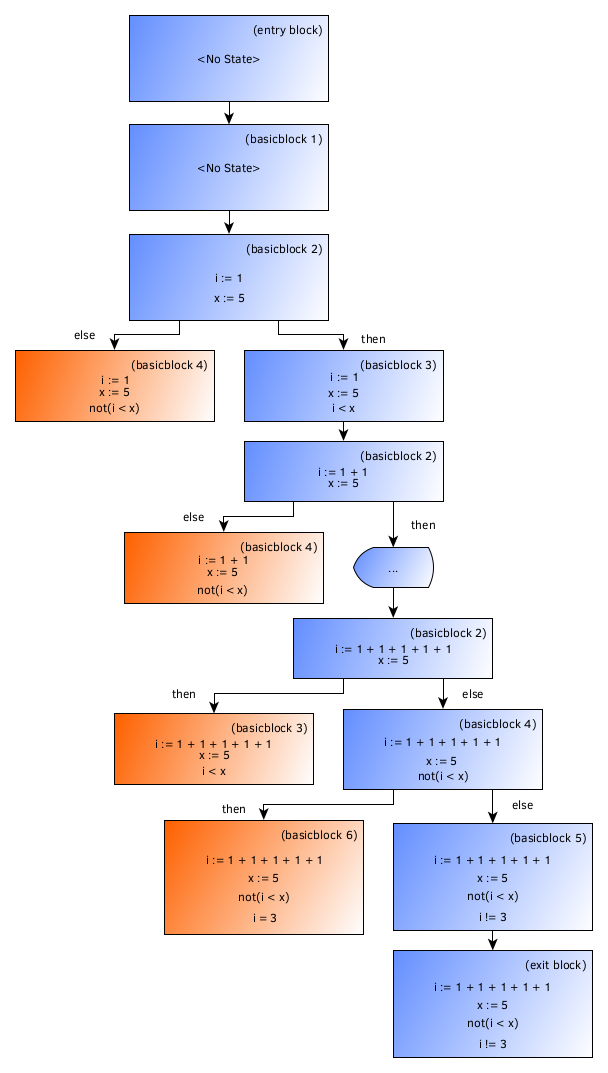
\includegraphics[width=0.6\textwidth]{basic-while}
	\caption{Analysis of example shown in Listing \ref{code:loop example 1} and Figure \ref{fig:loop example 1 cfg}. For each iteration the analysis checks if the condition of the loop finally evaluates to true until it does. Since the variable \emph{x} is known, there is only one feasible branch to follow.}
	\label{fig:loop example 1}
\end{figure}

\begin{program}[h!]
	\begin{GenericCode}
i := 1;
	
WHILE i < x DO
	i := i + 1;
END_WHILE;
	
IF i = 3 THEN
	x := 4;
END_IF;		\end{GenericCode}

\centering
\caption{Same as \ref{code:loop example 1}, but x is an input variable. Therefore it may be 3, so it could be reachable.}
\label{code:loop example 2}
\end{program}
\begin{figure}[h!]
	\centering
	% <1ms
	% 68
	% No violations
	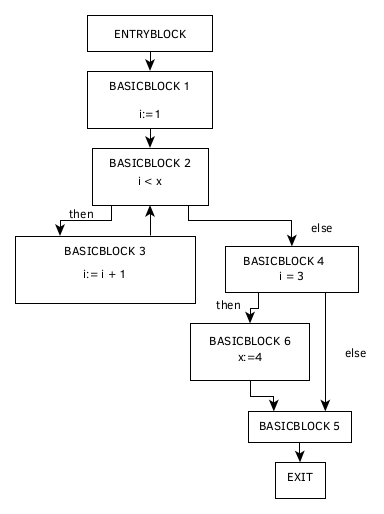
\includegraphics[width=0.6\textwidth]{basic-while-input-cfg}
	\caption{This CFG is almost identical to \ref{fig:loop example 1 cfg}, with the exception that the assignment in line 2 is missing.}
	\label{fig:loop example 2 cfg}
\end{figure}
\begin{figure}[h!]
	\centering
	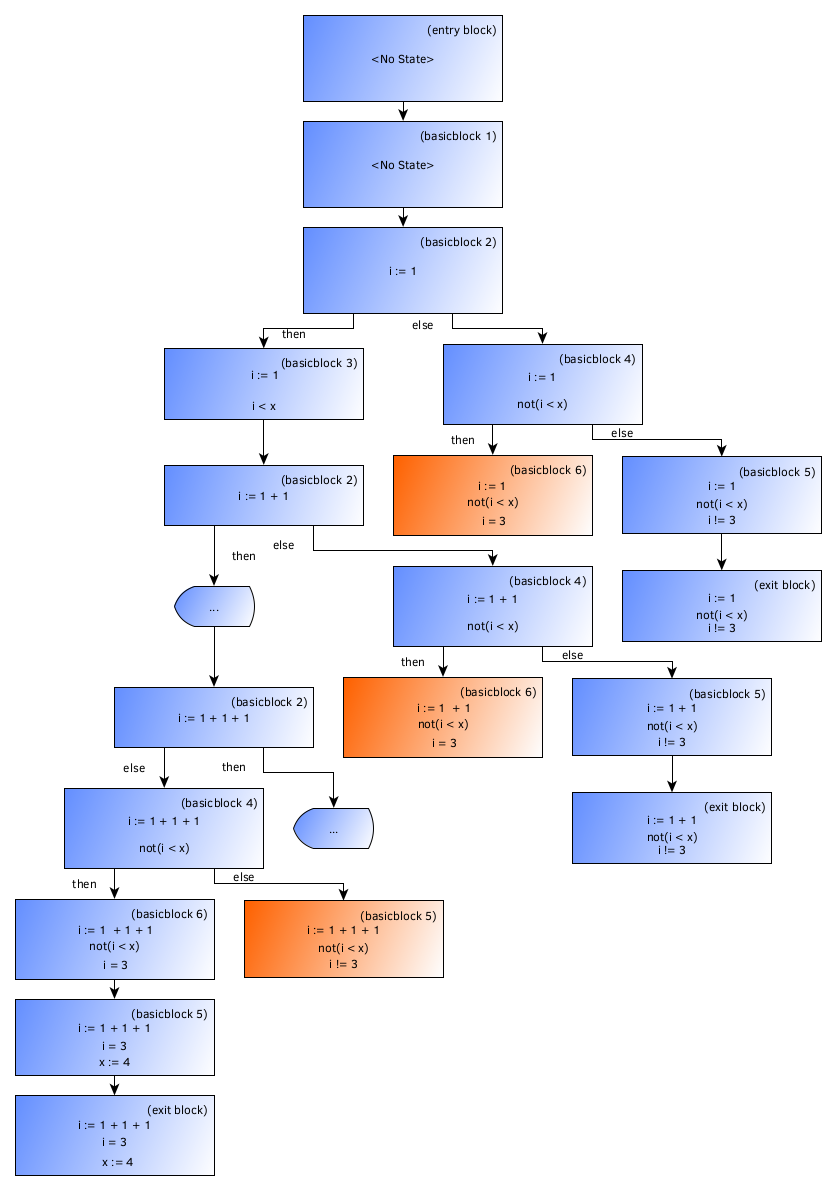
\includegraphics[width=0.8\textwidth]{basic-while-input}
	\caption{Analysis of example shown in Listing \ref{code:loop example 2} and Figure \ref{fig:loop example 2 cfg}. Since the value of \emph{x} is nondeterministic, every possible value has to be explored, in contrast to \ref{fig:loop example 1}. Without any type of early stopping, this analysis would try to calculate forever, as indicated by the rounded boxes. }
	\label{fig:loop example 2}
\end{figure}
\section{Function and Procedure Calls}
The example in Listing \ref{code:func test 1} was created to demonstrate how function and procedure calls are handled. The functionblock \emph{FooOutput} and \emph{algo1} of the instantiated algorithmblock are called. The functionblock \emph{FooOutput} takes three parameters. The first is an input parameter, which is passed by value, the second is an output parameter, possibly changing the value, and the last parameter is an in-out parameter, which may also change its value.
The algorithm \emph{algo1} has a similar declaration. The first parameter, declared as \emph{in1}, is an input parameter, the second is an in-out parameters, called \emph{in\_out1}, and the last, called \emph{out1}, is an out parameter.

After the first three assignments, the funcitonblock is called and therefore the variables \emph{tmp1} and \emph{tmp2} may change their value. As described in Section \ref{sub:handling procedure and function calls} this analysis is done intraprocedurally, meaning the concrete new values these variables hold are not evaluated, but become rather nondeterministic. This can be observed in Figure \ref{fig:func test 1}. The assignments and the procedure call are in basic block 1 (as seen in Figure \ref{fig:func test 1 cfg}), but in the following branches (in \ref{fig:func test 1}) do not contain the restrictions for the variables \emph{tmp1} and \emph{tmp2} anymore. Therefore the condition in line 7 may either be true or false.
Since \emph{tmp1} does not change,  the condition in line 11 will always evaluate to false, causing unreachable code in line 12 (basic block 5).

The procedure call in line 15 creates a nondeterministic state for the variables \emph{tmp1} and \emph{tmp3}, which means the condition in line 17 may evaluate to true or false.

The procedure call in line 21 has the same effect as the one before, but using named parameters (the parameters \emph{tmp1} and \emph{tmp3} switched position, but are handled the same as before).

The variable \emph{tmp2} does not change, but may hold value 2 when the prior condition in line 7 evaluated to true. Therefore the condition may be true, but does not have to be. Therefore the assignment in line 24 is reachable. 

Since the tools mentioned in Chapter \ref{cha:state of the art} only operate on Java source code, this example has to be converted to make a fair comparison.
When this example is converted to Java, the parameters have to be handled. Variables of primitive datatypes are passed by value, while others are passed by reference. Therefore a special class has to be introduced to simulate this behavior. 

None of the tools mentioned in Chapter \ref{cha:state of the art}, with maybe the exception of joogie, which could not be executed.


\begin{program}[h!]
	\begin{GenericCode}
tmp1 := 1;
tmp2 := 2;
tmp3 := 3;

FooOutput(tmp1, tmp2, tmp3);

IF tmp2 <> 2 AND tmp3 <> 3 THEN
	tmp2 := 2; // Reachable - could change
END_IF;

IF tmp1 <> 1 THEN
	tmp2 := 3; // Unreachable
END_IF;

ABFunc.algo1(tmp2, tmp1, tmp3);

IF tmp1 <> 1 AND tmp3 <> 1 THEN
	tmp2 := 3; // Reachable
END_IF;

ABFunc.algo1(out1 => tmp1, in1 := tmp2, in_out1 := tmp3);

IF tmp2 = 3 THEN
	tmp2 := 3; // Reachable
END_IF;	\end{GenericCode}
	\centering
	% 169ms
	% 31 
	% Violations 5
	\caption{Demonstrates intraprocedural analysis. The procedure  FooOutput declares the first parameter as an IN parameter and therefore has no effect on the variable, while the other two parameters are declared as OUT parameters and might change. Note that the analysis does not check if the out parameter will be mutated, so it will be counted as if it would have. ABFunc is an instantiated algorithm block, which is similar to a class, and declares the parameters of the procedure \emph{algo1} in the same order. Note that the second occurrence of this method call contains named parameters. \emph{out1} and \emph{in\_out3} may be mutated.}
	\label{code:func test 1}
\end{program}
\begin{figure}[h!]
	\centering
	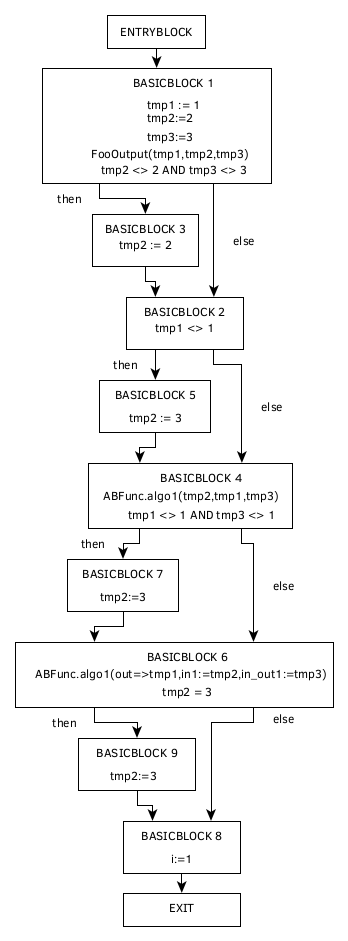
\includegraphics[width=0.5\textwidth]{easy-func-test-cfg}
	\caption{CFG of example shown in Listing \ref{code:func test 1}. It does not contain any loops, since all arrows point in the same direction, but does contain many branches, needed for the demonstration of this analysis.}
	\label{fig:func test 1 cfg}
\end{figure}
\begin{figure}[h!]
	\centering
	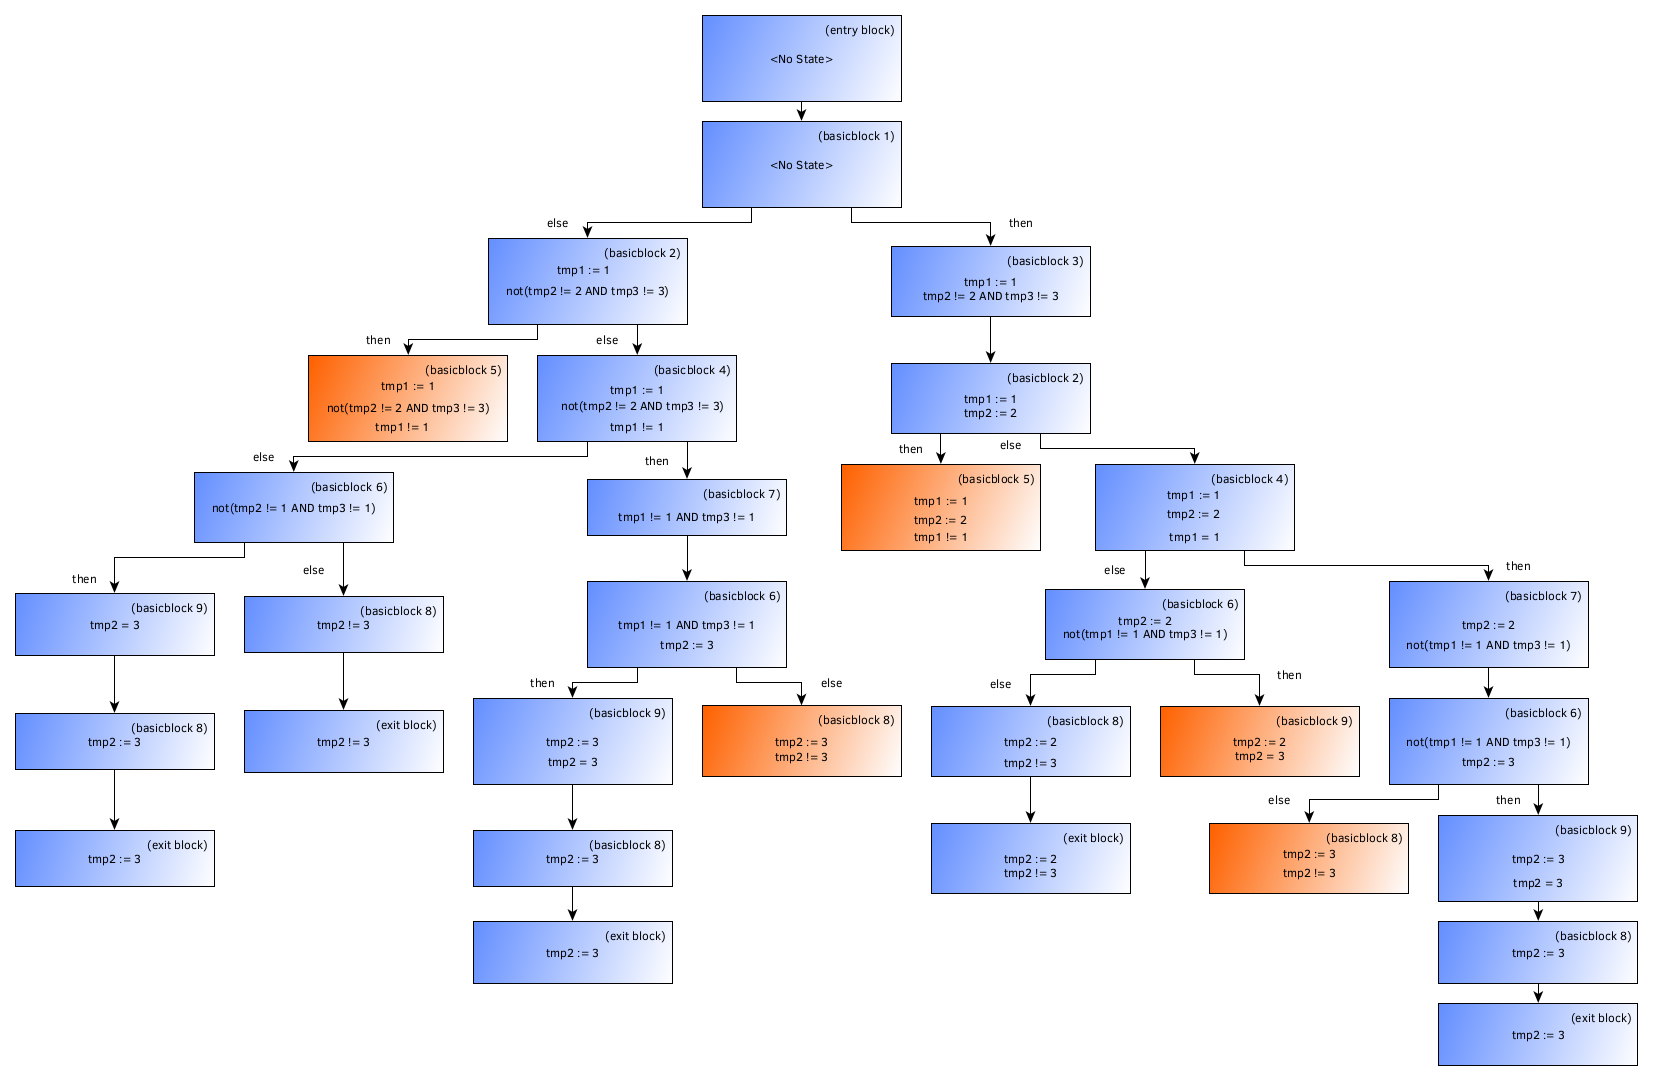
\includegraphics[width=1\textwidth]{easy-func-test}
	\caption{Analysis of example shown in Listing \ref{code:func test 1} and Figure \ref{fig:func test 1 cfg}. Function and procedure calls have been dissolved and reset the actual parameters passed as output variables to a nondeterministic state. This can be observed for example in the blocks after the second block (basic block 1), since the assignments to \emph{tmp2} and \emph{tmp3} are not shown in the following blocks.}
	\label{fig:func test 1}
\end{figure}

\section{Hard Example}
The example in Figure \ref{code:hard example 1} and Figure \ref{fig:hard example 1} was found in the literature \cite{Click_1995}. In this research paper it is stated:
\begin{quote}
	Neither
	simple constant
	propagation
	nor unreachable-code elimination
	discovers these facts because
	each analysis
	needs a fact
	that can only be discovered
	by the other.
\end{quote}
Since this implementation does not rely on constant propagation and does not simplify loops in any form, it should be detected. In this example shown in Listing \ref{code:hard example 1} the two important variables are \emph{x} and \emph{b}. The \emph{pred} variable could as well be a function, but is not of importance for this analysis. The first statement in the loop in line 4 always evaluates to false, since the value of variable \emph{x} is one and does never change. Therefore the condition in line 5 always evaluates to false and the statement in line 6 (or basicblock 4 in \ref{fig:hard example 1}) is unreachable. As Figure \ref{fig:hard example 1 cfg} shows, this analysis may never finish and therefore the implementation would not be able to find this instance of unreachable code. This can be circumvented by following the flow of a loop for a set amount of time as stated in Section \ref{sub:early stopping}. By doing so false positives could be reported, because during the analysis a loop could not have been evaluated often enough. When for example the repeat-until loop was replaced by a for loop and be evaluated exactly n times, the analysis could potentially evaluate this loop m times, where m is smaller than n. When also replacing the condition in line 5 so that it would evaluate to true in the last iteration, it could potentially not be analyzed correctly by the implementation.

Neither of the tools described in Chapter \ref{cha:state of the art} are able to find this kind of error.
This begs the question if a static code analysis tool must be capable to find this kind of error by expanding potentially enormous amounts of time and power necessary to find this edge cases. Other static code analysis tools do not even check multiple iterations of loops to save on execution time. Integrated development environments must deliver warnings for errors as fast as possible to guarantee a pleasant experience. Only separate tools, like sonarqube \cite{sonarqube}, could have the power to detect these edge cases. But even then bigger projects could contain many multiple loops, which could slow down this analysis significantly. Paired with multiple function and procedure calls the execution time could be too high to tolerate, with little extra information. As described in Section \ref{sub:problems and barriers} some sort of preprocessing could work to reduce execution time.

\begin{program}[h!]
	\begin{GenericCode}
x := 1;
	
REPEAT
	b := x <> 1;
	IF b = TRUE THEN
		x := 2;
	END_IF;    
UNTIL pred
END_REPEAT;	\end{GenericCode}
	\centering
	\caption{This example cannot be analyzed correctly by existing static code analysis tools. Since the variable \emph{b}, relevant for the condition in line 5, is dependent on x, which does only change when b would be true in line 4, line 6 becomes unreachable. }
	\label{code:hard example 1}	
\end{program}

\begin{figure}[hbt!]
	% 20ms
	% 47
	% Violation Block 4
	\centering
	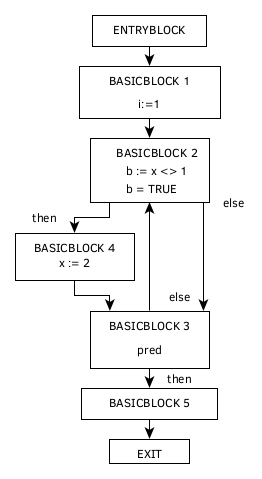
\includegraphics[width=0.4\textwidth]{hard-example-cfg}
	\caption{CFG of example shown in Listing \ref{code:hard example 1}. Since the condition in basicblock 2 never evaluates to true, basicblock 4 becomes unreachable.}
	\label{fig:hard example 1}
\end{figure}
\begin{figure}[hbt!]
	\centering
	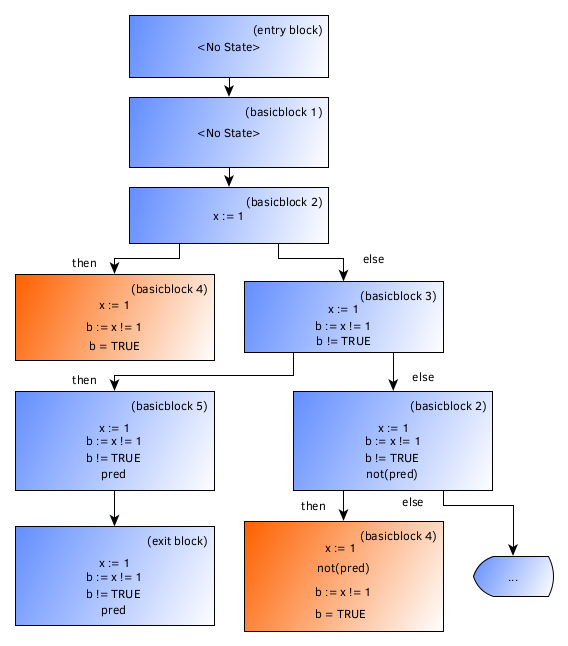
\includegraphics[width=0.7\textwidth]{hard-example}
	\caption{Analysis of example shown in Listing \ref{code:hard example 1} and Figure \ref{fig:hard example 1}. This analysis would run forever without the correct configuration. After a defined amount of iterations the analysis stops and reports, which blocks are unreachable. This may work for this particular example, but could cause problems otherwise, since the condition of the loop is not depend on any variables, that may change inside the body of the loop or any variable is relevant outside the loop.}
	\label{fig:hard example 1 cfg}
\end{figure}

\section{Overview of results}
\label{sec:overview of results}
In Table \ref{tab:runtime-overview} the runtime of the analysis of each example can be compared to others. The collected metrics contain median, minimum and maximum runtime as well as the analyzed blocks. 
Each example was run exactly 100 times on a machine with a Intel(R) Core(TM) i7-8665U CPU @ 1.90 GHz, 2112 Mhz, 4 Cores with 8 Logical Processors. 
Interestingly the number of analyzed block does have a direct effect on runtime. This may be due to the reason that some of the analyzed blocks were not completely evaluated, at least the example described in Section \ref{sec:loops}, because the analysis stops prematurely. Handling of function and procedure calls is tedious, because the information of the called function/procedure takes time. In this implementation all functions and procedures are stored in a database and for each call in the source code the information has to be looked up.

\begin{table}[h!]
\begin{tabular}{lcccc}
Example                      & \multicolumn{1}{c}{\begin{tabular}[c]{@{}c@{}}Median\\ Runtime\end{tabular}} & \multicolumn{1}{c}{\begin{tabular}[c]{@{}c@{}}Minimum \\ Runtime\end{tabular}} & \multicolumn{1}{c}{\begin{tabular}[c]{@{}c@{}}Maximum\\ Runtime\end{tabular}} & \multicolumn{1}{c}{\begin{tabular}[c]{@{}c@{}}\# \\ of analyzed blocks\end{tabular}} \\
\hline
Infeasible Code Example                & 23ms                                                                         & 21ms                                                                           & 31ms                                                                          & 17                                                                                   \\
Loops (No Input Variable)    & 23ms                                                                         & 22ms                                                                           & 34ms                                                                          & 20                                                                                   \\
Loops (With Input Variable)  & 1ms                                                                          & 1ms                                                                 & 2ms                                                                           & 68                                                                                   \\
Function and Procedure Calls & 511ms                                                                        & 492ms                                                                          & 841ms                                                                         & 31                                                                                   \\
Hard Example                 & 26ms                                                                         & 25ms                                                                           & 34ms                                                                          & 47                                                                                  
\end{tabular}
	\caption{Overview of the tested examples and their minimum, maximum and median runtime. One hundred runs per example were executed.}
	\label{tab:runtime-overview}
\end{table}



